\documentclass[10pt]{article}
\usepackage{multicol}
\usepackage[margin=0.75in]{geometry}
\usepackage{hyperref}
\hypersetup{
    colorlinks=true,
    linkcolor=blue,
    filecolor=magenta,      
    urlcolor=cyan,
}
\usepackage{graphicx}
\begin{document}

\title{
  A Fast, Multi-Threaded, \\
  Master-Worker Web Server \\
  \Large Proof of Concept in Go
}
  
\author{
  Robert Carney, Donald Hamnett, and Nicholas Vann \\
  Northeastern University \\
  CS5600 Fall 2018 \\
  Final Project 
}
\maketitle
\section*{Abstract}
\begin{multicols}{2}

\par
With the exponential increase in the use of the web and distributed computing in the last quarter century, the search for a fast and reliable web server is more important than ever.  One approach to achieving speed and reliability is a master-worker model, where a master process is given few responsibilities, and delegates the workload to a pool of separate processes, the workers.  Our project aimed to implement a proof of concept using our own flavor of the master-worker model.  When deciding which tool was best suited for this job, we decided to develop our solution in Go (Golang). Go was developed by Rob Pike and Ken Thompson (of Bell Labs/Unix/C lore) on behalf of Google.  Its goal was to create a developer-friendly, systems-level language which made some of the more involved tasks of multi-threaded programming easier than in C or C++.  Though created with Google's internal use in mind, Go has become a popular choice among several industry players for implementing micro services. We were able to achieve our goal using this previously unfamiliar language, with some interesting benchmarking results against the default configuration of one of the most widely used web servers in history, the Apache2 server.
\section*{Why Go?}
\par
The advantages of Go for a web project are largely due to who it was created for and when it was created.  
\subsection*{Built for Google}
\par
Google is one of the largest companies in the world, and its business functionality is heavily reliant on the internet and web services.  As such, one would expect that any language which they commissioned for their own use would have robust and well integrated HTTP and TCP/IP standard library support.  We found this to indeed be the case with Go, and when comparing documentation, APIs, and code examples across commonly used languages, it was clear that Go would be the quickest to get up to speed with in order to begin our web server implementation.  
\subsection*{Built in the Age of Concurrency}
\par
Go was created within the last decade, when multi-core CPUs were becoming the norm and Moore's Law was coming to a close.  Due to the increase in cores, and decrease in the year-to-year increase of core speed, the software development community has largely turned to writing parallel and multi-threaded programs as a solution to improving performance.  With this in mind, instead of relying on external libraries for managing threads, Go was built with native multi-threading support. Its threading model is based on lightweight threads, or "go-routines" (a tongue-in-cheek nod to co-routines), and channels, which are thread-safe queues suitable to atomically access shared data between threads. This native multi-threading support leaves less concurrency management responsibility on the developer, handling the details behind the scenes.
\section*{Design}
\par
Our web server implementation is based on the master-worker model, where one "master" process handles external communication and general management responsibilities, and a configurable number of "workers" actually serve the files, carrying out requests from the master and communicating back the results.
\end{multicols}
\begin{figure}
\centering
        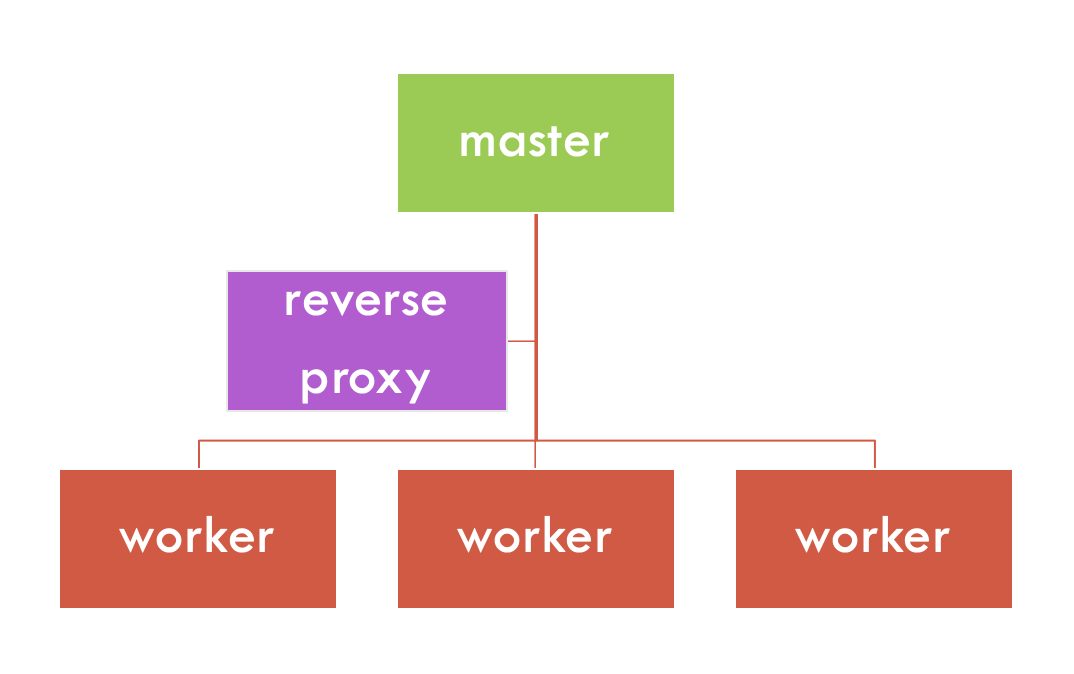
\includegraphics[totalheight=9cm]{./images/masterworker.png}
        \caption{Our master-worker model}
\end{figure}
\begin{multicols}{2}
\subsection*{Master Responsibilities}
\begin{itemize}
\item 
\textbf{Reading Configuration:}
\par
On initialization, the master reads a JSON configuration with information such as the base file directory to serve, the host and ports of workers, and its own port to serve.
\item
\textbf{Spawning Workers:}
\par
The master spawns workers, passing configuration values as command-line arguments.
\item
\textbf{Load Balancing:}
\par
Using a reverse proxy with the workers, the master sends and receives messages from clients, to the workers, and subsequently from the workers to the clients.
\item
\textbf{Health-Checking:}
\par
Another go-routine of the master issues periodic health-checks to the workers, and if unhealthy, kills and restarts the unhealthy process.
\item
\textbf{Graceful Shutdown:}
\par
Upon receiving an interrupt to kill the master, it also kills the worker processes.
\end{itemize}
\subsection*{Worker Responsibilities}
\begin{itemize}
\item
\textbf{Listen for File Requests:}
\par
Set up and listen on endpoints for each path within the base directory.
\item
\textbf{Serve Requested Files:}
\par
Write file contents as response when receiving a request on an endpoint.
\item
\textbf{Caching:}
\par
When a file is accessed, save it in a temporary cache to serve more quickly if requested again, increasing performance in the case of temporal locality.
\item
\textbf{Respond to Health-Checks:}
\par
Respond to requests to the health-check endpoint with StatusOK, if healthy, and StatusUnavailable otherwise. The worker always sent a healthy response in our POC, but this can be extended to more complex situations, so we included atomic boolean operations to set the worker as healthy or unhealthy.
\end{itemize}
\end{multicols}
\pagebreak
\begin{multicols}{2}
\section*{Benchmarking}
\par
In order to test our server's performance, we benchmarked against Apache2 server.
\subsection*{Benchmarking Parameters}
\begin{itemize}
\item
Used \textit{Apache Benchmark} command-line application
\item
Sent $5000$ total requests
\item
Set request concurrency to $500$
\item
Used Apache2's default configuration
\item
Tested our server with $2$, $10$, and $100$ workers
\end{itemize}
\subsection*{Benchmarking Results}
\par
Apache2 server consistently beat our server's performance up until approximately $4800$, requests, where our server beat Apache2.  At this point, Apache2's response time increased exponentially, and actually left some requests unfulfilled.  Conversely, our server succeeded in fulfilling all requests. Our server's performance also increased in direct proportionality to the number of worker servers. While we were pleased with the results, they may be misleading. This is because the default configuration for Apache2 is single threaded, while ours was taking advantage of the full CPU performance.  It is questionable whether we could best Apache2 with a configuration better tuned for the testing hardware. Regardless, we were pleased to potentially find a use case where our server performed comparatively well to an established entity such as Apache2.
\end{multicols}
\begin{figure}[h]
\centering
        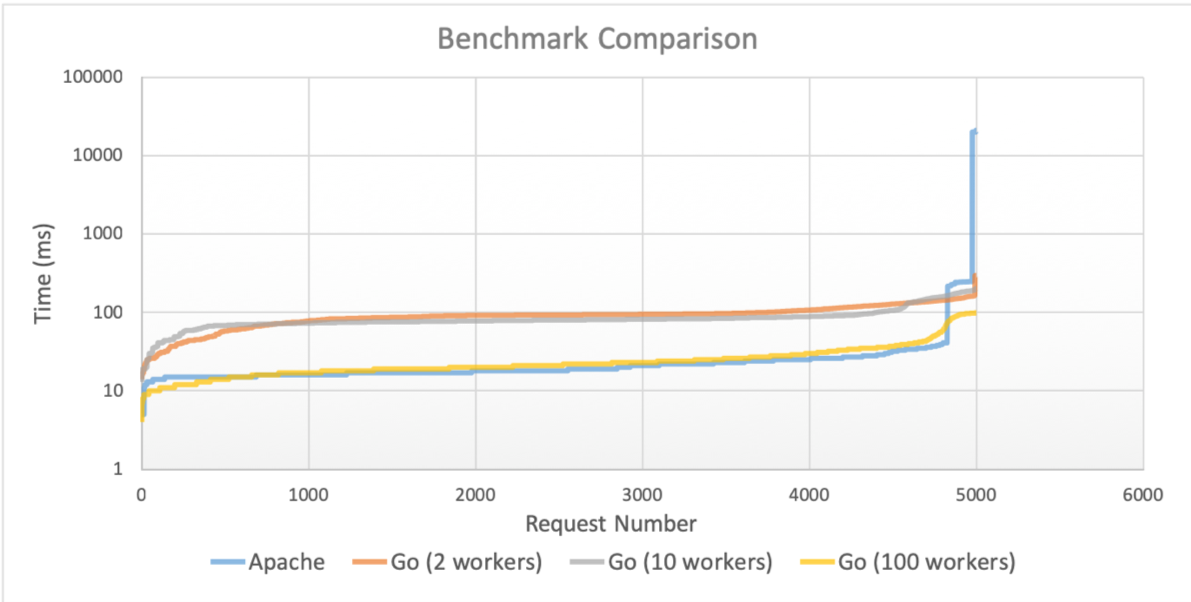
\includegraphics[width=16cm]{./images/graph.png}
        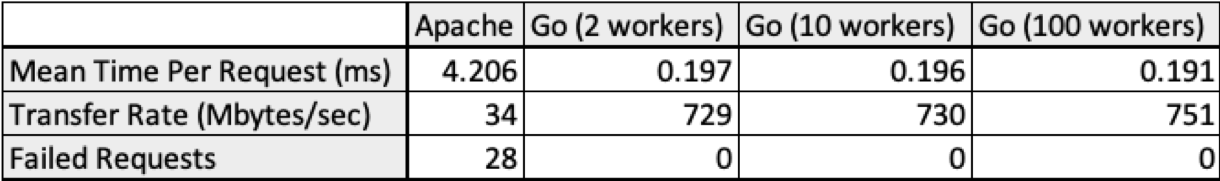
\includegraphics[width=16cm]{./images/table.png}
        \caption{Benchmarking Results}
\end{figure}
\pagebreak
\begin{multicols*}{2}
\section*{Future Improvements}
\par
Seeing as this was a proof of concept, there are several future improvements we would make if continuing development on this project. These include, but are not limited to, the following:
\begin{itemize}
\item
Extend to a distributed protocol to work on multiple machines
\item
Add further options for configurations to give users more control
\item
Implement daemons to manage workers on distributed machines
\item
Incorporate distributed caching and storage
\item
Add measures for increased security
\end{itemize}
\section*{Find us on Github!}
\par
To browse our Github repository visit \href{https://github.com/robcarney/gows}{robcarney/gows}.
\end{multicols*}
\end{document}
